\documentclass[11pt]{article}
\usepackage[finnish]{babel}
\usepackage[utf8]{inputenc}
\usepackage{graphicx}
\usepackage{float}
\usepackage{epstopdf}
\usepackage{tikz}
\definecolor{sininen}{HTML}{CCE6FF}
\definecolor{vihrea}{HTML}{CCFFCC}
\definecolor{keltainen}{HTML}{FFEFCC}
\definecolor{punainen}{HTML}{FFC0CB}
\definecolor{valkoinen}{HTML}{FFFFFF}
\definecolor{harmaa1}{rgb}{0.9, 0.9, 0.9}
\definecolor{harmaa2}{rgb}{0.8, 0.8, 0.8}
\definecolor{harmaa3}{rgb}{0.7, 0.7, 0.7}
\renewcommand*{\familydefault}{\sfdefault}
\title{\textbf{Keskustelufoorumi}\\ \small{dokumentaatio}}
\author{John Lång}
\date{3.6.2014}
\begin{document}

\maketitle

\thispagestyle{empty}
%Tehty \LaTeX:lla.

\newpage
%Pystyyköhän tälle jotenkin antamaan oman suomenkielisen otsikon?
\tableofcontents
\thispagestyle{empty}

\newpage

\section{Johdanto}
	Tämän projektin tarkoituksena on toteuttaa perinteinen web-pohjainen keskus-telufoorumi. Ohjelmiston
	avulla internetin käyttäjät voivat perustaa omia (yleen-sä tiettyyn aihepiiriin keskittyviä) yhteisöjään
	joihin jokainen rekisteröity jäsen voi tuottaa omaa sisältöään (yhteisön sääntöjen mukaisesti). Lisäksi
	projektin tavoitteena on luonnollisesti tarjota mahdollisimman tehokkaat ja käyttäjäystä-välliset työkalut 
	foorumin ylläpidosta sekä moderoinnista vastaaville yhteisön jäsenille, jotta he voisivat suorittaa
	tehtäväänsä	tarkoituksenmukaisesti.
		
	Aion toteuttaa projektin käyttämällä java-ohjelmointikieltä Netbeans IDE:llä sekä (Tietojenkäsittelytieteen laitoksen
	palvelimille asennettuja) PostgreSQL-tietokantaa ja Apache Tomcat -http-palvelinta. Loppukäyttäjälle
	näkyvän sivuston ulkoasun aion toteuttaa HTML 5- sekä mahdollisesti CSS-kielten avulla. Tavoitteenani
	on myös salata mahdollisimman suuri osa foorumin tietoliikenteestä HTTPS-protokollan avulla.
	
	Itse tämän dokumentin laatimisessa olen käyttänyt hyväkseni avoimen lähde-koodin ohjelmistoja.
	Gummi:lla olen tehnyt itse pdf-tiedoston, Dialla (UML-)\\ kaaviot, LibreOffice Calc:lla käyttötapausmallin
	taulukot, sekä Inkscapella muuttanut nämä kuvat eps-formaattiin pdf-tiedostoon liittämistä varten.
	
	Pyrkimyksenäni on pitää järjestelmän vaatima asennustyö minimissä enkä siksi aio käyttää muita kun kielten
	standardikirjastoja sekä mainitsemiani palvelin-ohjelmistoja. Lisäksi aion tehdä ohjelmistostani mahdollisimman näkymättömän loppukäyttäjälle
	siten, ettei foorumin käyttäminen edellytä mitään selainliitän-näisiä tai javascriptin käyttöä. Luultavasti
	joudun kuitenkin (valitettavasti) käyt-tämään evästeitä esimerkiksi käyttäjäkohtaisten istunto- ja
	asetustietojen tallentamiseen.
	
	Olen valinnut projektilleni MIT-lisenssin, joka löytyy juurihakemiston tiedostosta LICENCE.
	% Tämän voisi varmaan mainita myös README.md:ssä
\newpage

\section{Yleiskuva}
	\subsection{Keskustelufoorumi}
		Keskustelufoorumi koostuu erilaisista lomakkeista ja työkaluista, joiden avulla järjestelmän tilaa
		muokataan, sekä tasopohjaisesta pääsynvalvonnasta neljällä eri \emph{käyttäjätasolla}.\footnote{
		Myöhemmin saatan ehkä lisätä myös käyttäjäryhmät, joiden perusteella voitaisiin valvoa
		pääsyä eri keskustelualueille saman kategorian käyttäjätunnusten keskuudessa.}
	
	\subsection{Käyttäjätasot}
		% Mitäpä jos olisi sellainen "puheoikeudeton" käyttäjätaso jonka käyttäjät saisivata vain käyttää
		% hakutoimintoja?
		Käyttäjätasot ovat \emph{vierailija}, \emph{jäsen}, \emph{moderaattori} ja \emph{ylläpitäjä}.
		Tasoihin liittyvät käyttöoikeudet ovat sisäkkäisiä siten, että vierailijalla on kaikkein suppeimmat
		ja ylläpitäjällä laajimmat käyttöoikeudet. Toisin sanoen ylläpitäjän oikeuksiin sisältyy kaikkien
		muiden tasojen oikeudet. Ylläpitäjä on keskustelufoorumin käyttöönoton suorittava henkilö. Alla on
		Vennin kaavio käyttäjätasoista.
	
		\begin{figure}[H]
			\vspace{1cm}
			\centering
			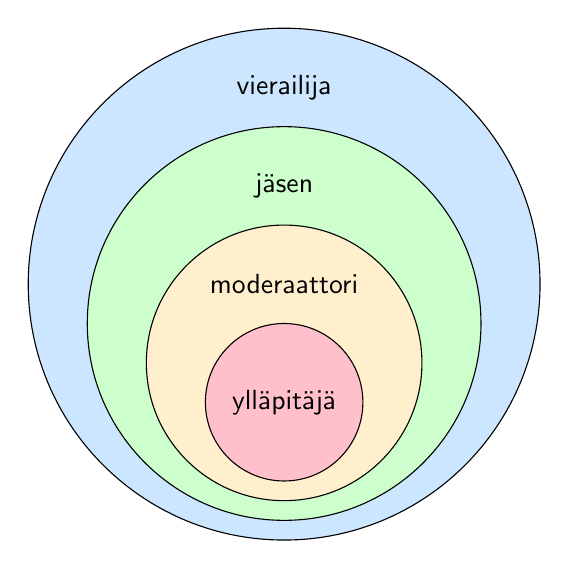
\begin{tikzpicture}
				\draw[fill=sininen] (0,1.5) circle(3.25);
				\draw[fill=vihrea] (0,1) circle(2.5);
				\draw[fill=keltainen] (0,0.5) circle(1.75);
				\draw[fill=punainen] circle(1);
				\node at (0,0) {ylläpitäjä};
				\node at (0,1.5) {moderaattori};
				\node at (0,2.75) {jäsen};
				\node at (0,4) {vierailija};
			\end{tikzpicture}\\
			\caption{Käyttäjätasot}
		\end{figure}
	
	\newpage
	\subsection{Rakenne ja toiminnot}
		Foorumin toiminnallisuuden ytimessä ovat käyttäjien tuottamaa sisältöä säilövät
		\emph{ketjut}\footnote{Käytän ketjusta myös synonyymiä \emph{viestiketju}.}, jotka
		sijaitsevat \emph{keskustelualueilla}. Lähtökohtaisesti kuka tahansa kes-kustelufoorumin web-sivustolla
		surffaava käyttäjä eli vierailija voi \emph{selata} keskuste-lualueita ja lukea niissä olevien ketjujen
		\emph{viestejä}.\footnote{
		Tavoitteenani on luoda ensin vain litteä hierarkia sisältäen yhden tasoisia keskustelualueita,
		joissa on vierailijoille näkyviä tavallisia ketjuja. Jos aikaa jää, saatan myös toteuttaa esimerkiksi
		sisäkkäisiä ja vierailijoilta piilotettuja keskustelualueita.}
		Lisäksi vierailija voi rekis-teröidä itselleen käyttäjätunnuksen.	
	
		\begin{figure}[H]
			\centering
			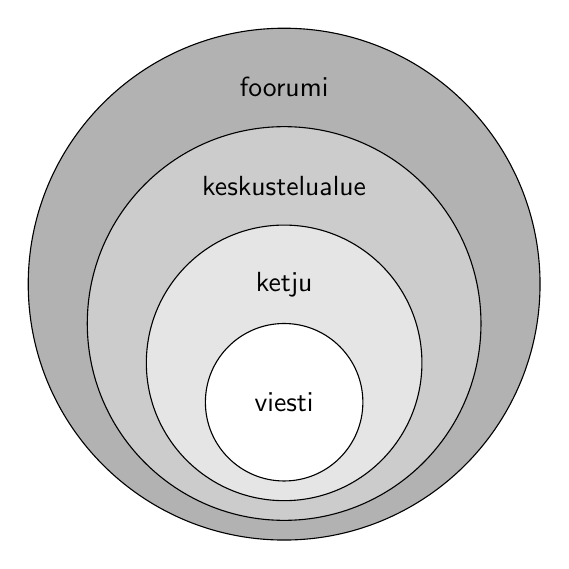
\begin{tikzpicture}
				\draw[fill=harmaa3] (0,1.5) circle(3.25);
				\draw[fill=harmaa2] (0,1) circle(2.5);
				\draw[fill=harmaa1] (0,0.5) circle(1.75);
				\draw[fill=valkoinen] circle(1);
				\node at (0,0) {viesti};
				\node at (0,1.5) {ketju};
				\node at (0,2.75) {keskustelualue};
				\node at (0,4) {foorumi};
			\end{tikzpicture}\\
			\caption{Foorumin rakenne}
		\end{figure}
	
		Jokainen rekisteröity käyttäjä eli jäsen voi aloittaa uuden ketjun sekä lisätä, muokata ja poistaa
		omia viestejään lukitsemattomissa ketjuissa. Näistä operaa-tioista käytän yhteisesti ilmausta
		\emph{viestitoiminnot}. Viestitoimintojen lisäksi jäse-net voivat käyttää \emph{hakutoimintoa}
		ketjujen ja viestien etsimiseen sekä muokata muille näytettäviä tietoja \emph{käyttäjätunnustoiminnoissa}. On syytä huomata että jäsentason käyttöoikeudet siis liittyvät
		\emph{käyttäjätunnuksiin} eli niiden käyttö edellyttää \emph{sisäänkirjautumista}.
	
		Moderaattorit ovat laajemmilla oikeuksilla toimivia
		käyttäjiä jotka voivat käsitellä mitä tahansa ketjun viestiä sekä lukita ja avata ketjun taikka siirtää
		sen toiselle keskustelualueelle.\footnote{Näin alkuvaiheessa en aio luvata mitään hienompia
		ominaisuuksia, kuten esimerkiksi ketjun määrittäminen \emph{tiedotteeksi} (joka saisi ketjun näkymään
		keskustelualueen listauksessa ennen tavallisia ketjuja).}
		Näistä toiminnoista käytän nimitystä \emph{moderointi}.
		Moderaattorien toimenkuvana on pitää huolta siitä että ketjujen ja viestien sisäl-tö vastaa foorumin
		tarkoitusta.\footnote{Foorumin tarkoitutksesta päättää ylläpitäjä ja siten asia on projektini
		aihealueen ulkopuolella.}
		Moderoinnin lisäksi moderaattoreilla on oikeus antaa \emph{porttikieltoja} jäsenille. Porttikiellot
		estävät sisäänkirjautumisen ja kohdistuvat käyttäjätunnuksiin (ei esimerkiksi IP-osoitteisiin, sillä
		niiden estäminen ei ole tehokasta ja voi haitata sivullisia).
	
		Viimeinen käyttäjätaso on ylläpitäjä. Ylläpitäjät voivat poistaa käyttäjätun-nuksen sekä korottaa taikka
		alentaa sen tasoa. Näissä toiminnoissa on kyse \emph{käyttäjätunnusten hallinnasta}. Lisäksi ylläpitäjä
		voi \emph{hallita keskustelualueita} eli perustaa, muokata tai poistaa keskustelualueen.
	
	\subsection{Käyttötapaukset}
		Edellä esitettyä vastaa seuraava käyttötapauskaavio:
		\begin{figure}[H]
			\centering
			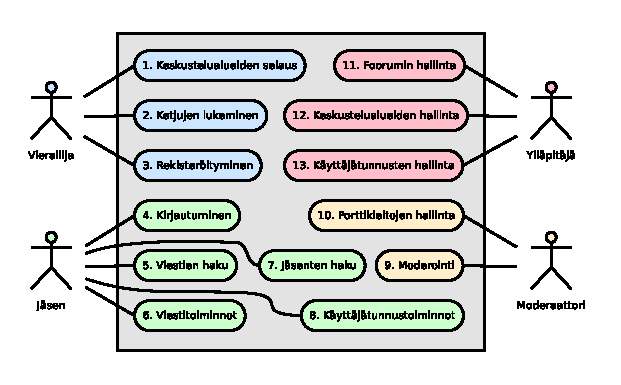
\includegraphics[trim = 7mm 0mm 0mm 0mm,scale=1.5]{kayttotapauskaavio.eps}\\
			\caption{Käyttötapauskaavio}
		\end{figure}
	
		Luettelen seuraavaksi maineikasta Alistair Cockburnin käyttötapausmallia\footnote{
		[Linkki tulossa...]}
		vapaasti mukaillen ohjelmistoni tärkeimmät käyttötapaukset.
	
		Seuraavat yhdeksän sivua sisältävät siis projektin käyttötapausmallit tauluk-komuotoisessa esityksessä.
	
		Selkeyden vuoksi olen käyttänyt taulukoissa samaa värikoodauta kuin käyttö-tapauskaavioissa erottamaan
		eri käyttäjätasojen käyttötapaukset. Olen myös merkinnyt tähdellä (*) ne käyttötapausten vaiheet,
		jotka ovat valinnaisia. Valinnaisen vaiheen voi jättää kokonaan tekemättä. Jos valinnainen vaihe
		sisältää syötteen antamista, niin käyttäjä voi antaa tyhjän syötteen. Jos valinnainen vaihe ohitetaan,
		ei siltä osin muuteta tietokannassa olemassaolevia tietoja. (Toi-saalta tyhjä syöte tyhjentää jonkin
		kentän arvon sitä vastaavassa tietokannan monikon attribuutissa ja merkitsee siten eri asiaa kuin
		vaiheen ohittaminen).\footnote{Lisäksi käyttötapauksessa 3 on syytä huomata, että käyttäjätunnuksen
		kirjautumisnimi määräytyy käyttäjätunnusta rekisteröitäessä eikä sitä voi jälkikäteen vaihtaa.}
	
		\newpage
		\pagestyle{empty}
		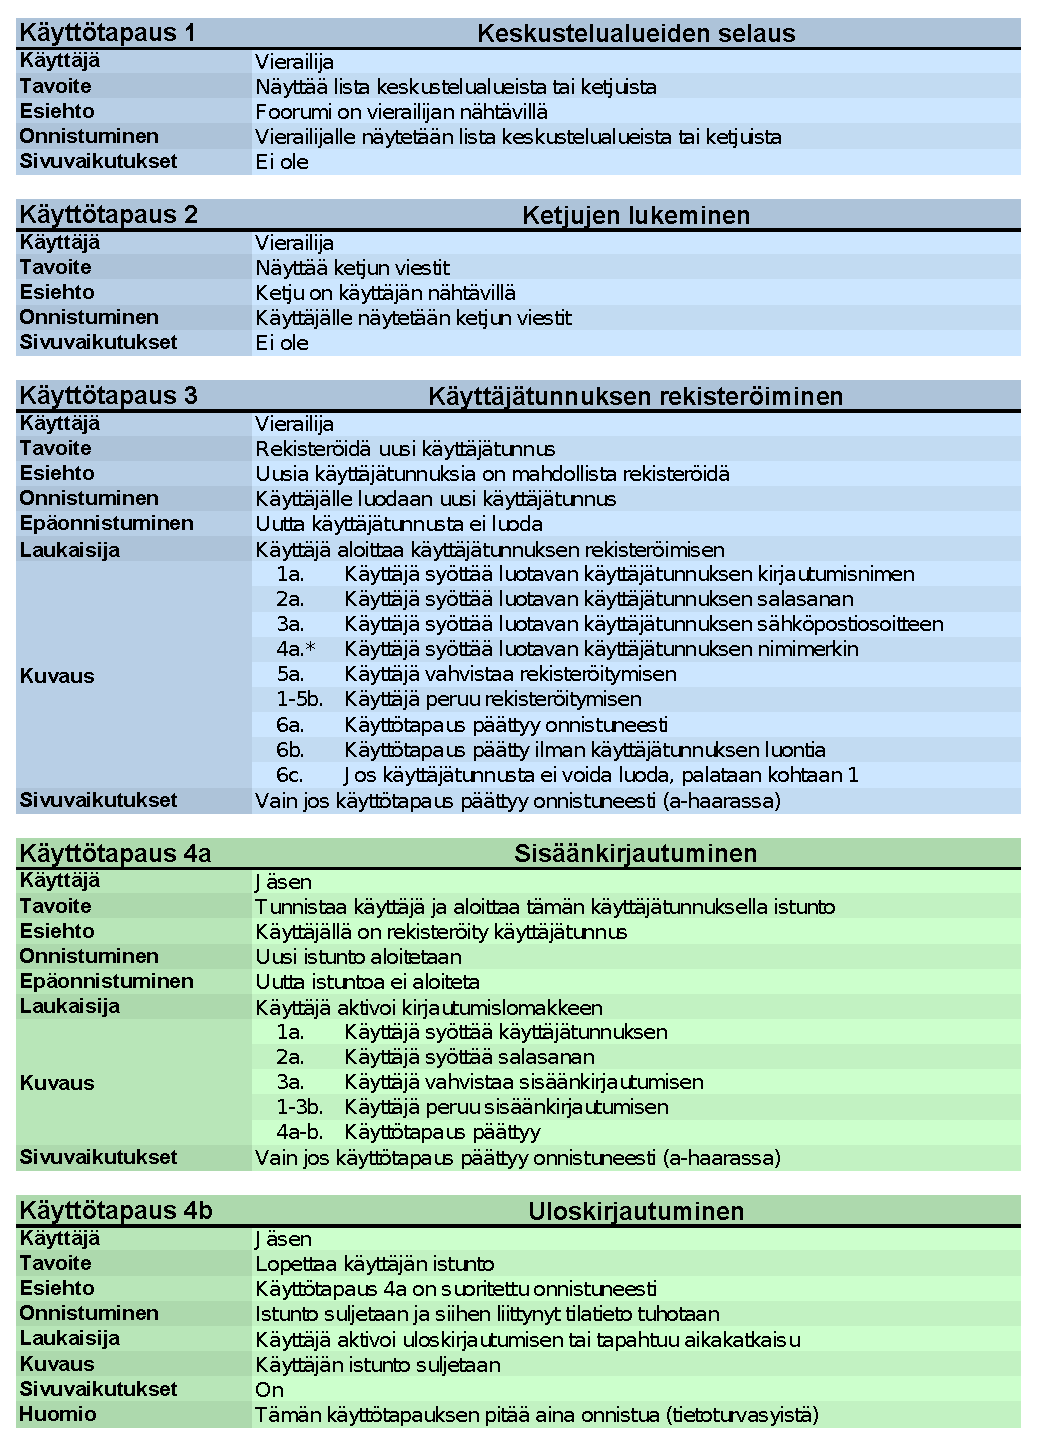
\includegraphics[trim = 27mm 0mm 0mm 25mm]{kayttotapausmalli-sivu-1.eps}\\
		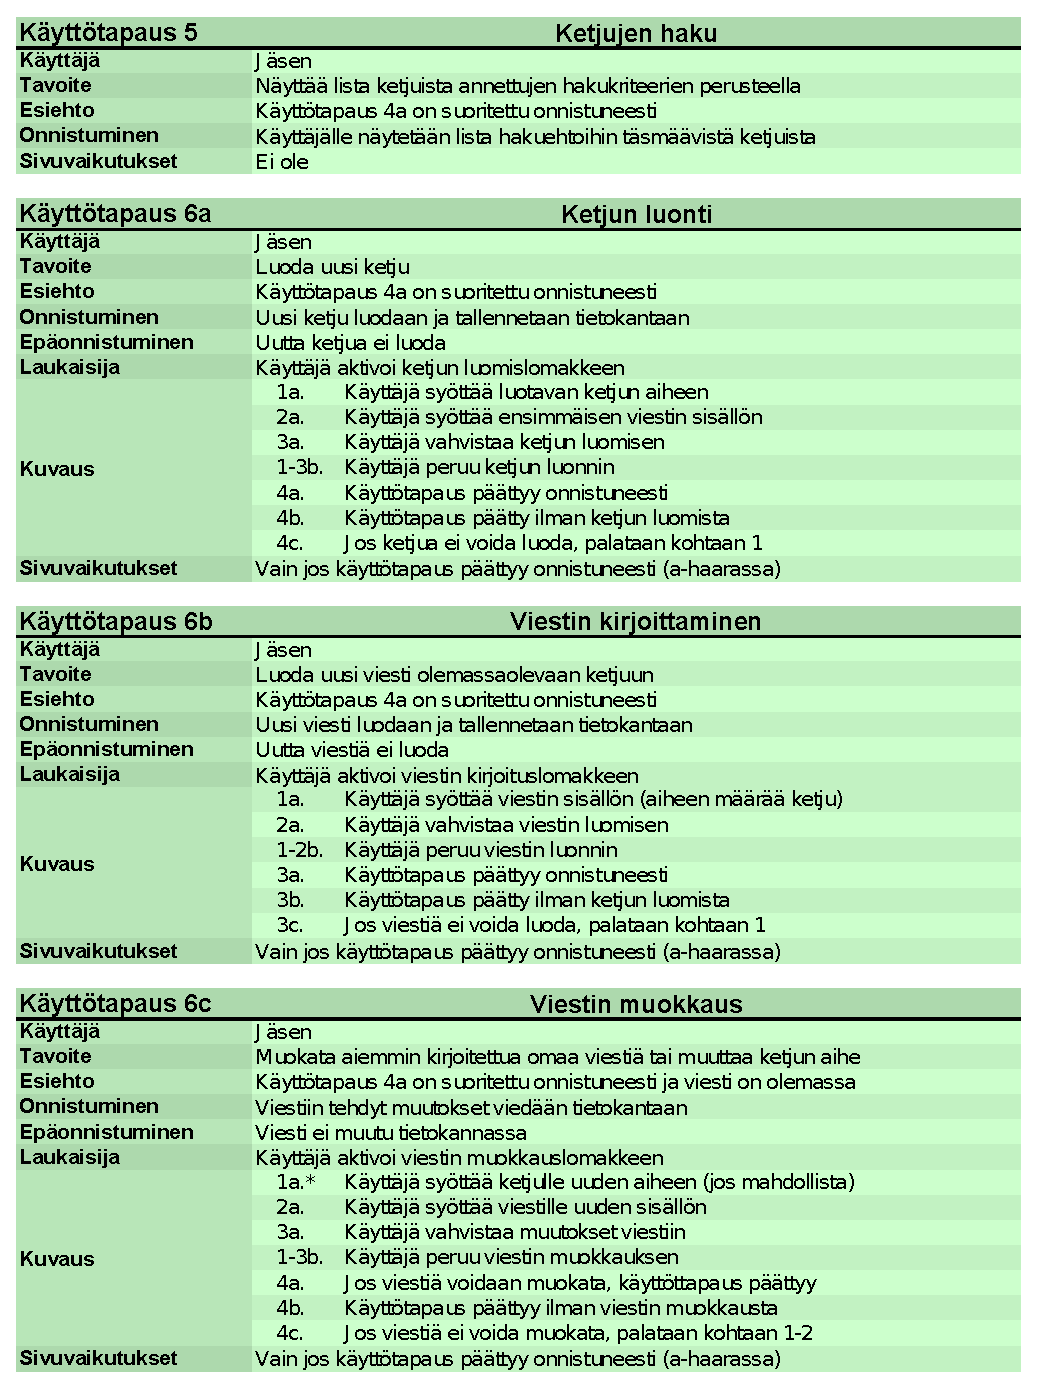
\includegraphics[trim = 21mm 0mm 0mm 25mm]{kayttotapausmalli-sivu-2.eps}\\
		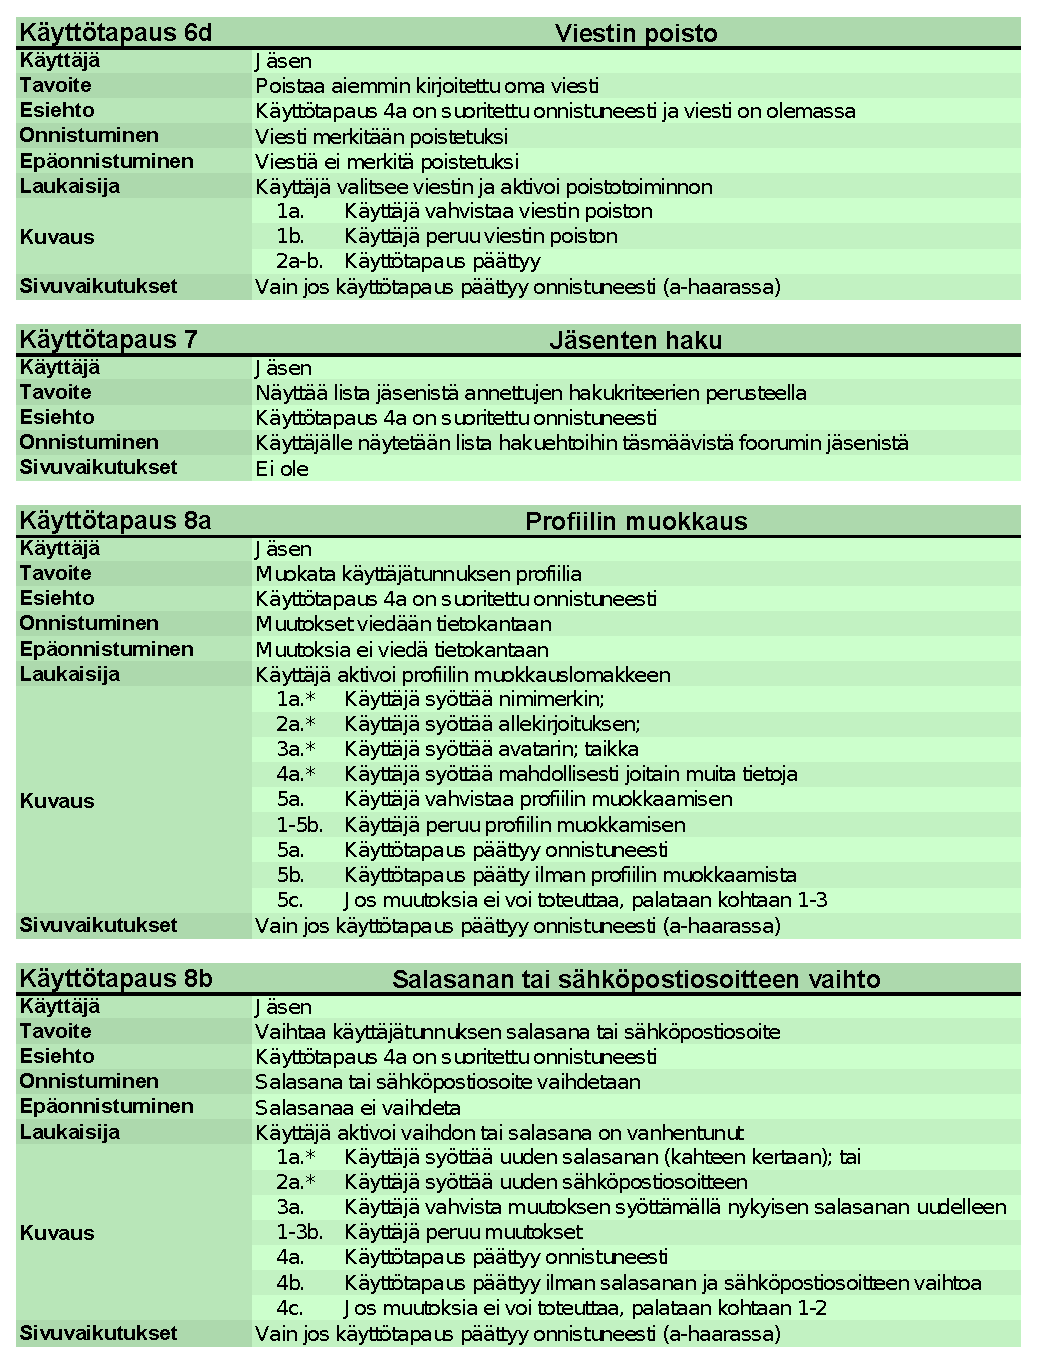
\includegraphics[trim = 21mm 0mm 0mm 25mm]{kayttotapausmalli-sivu-3.eps}\\
		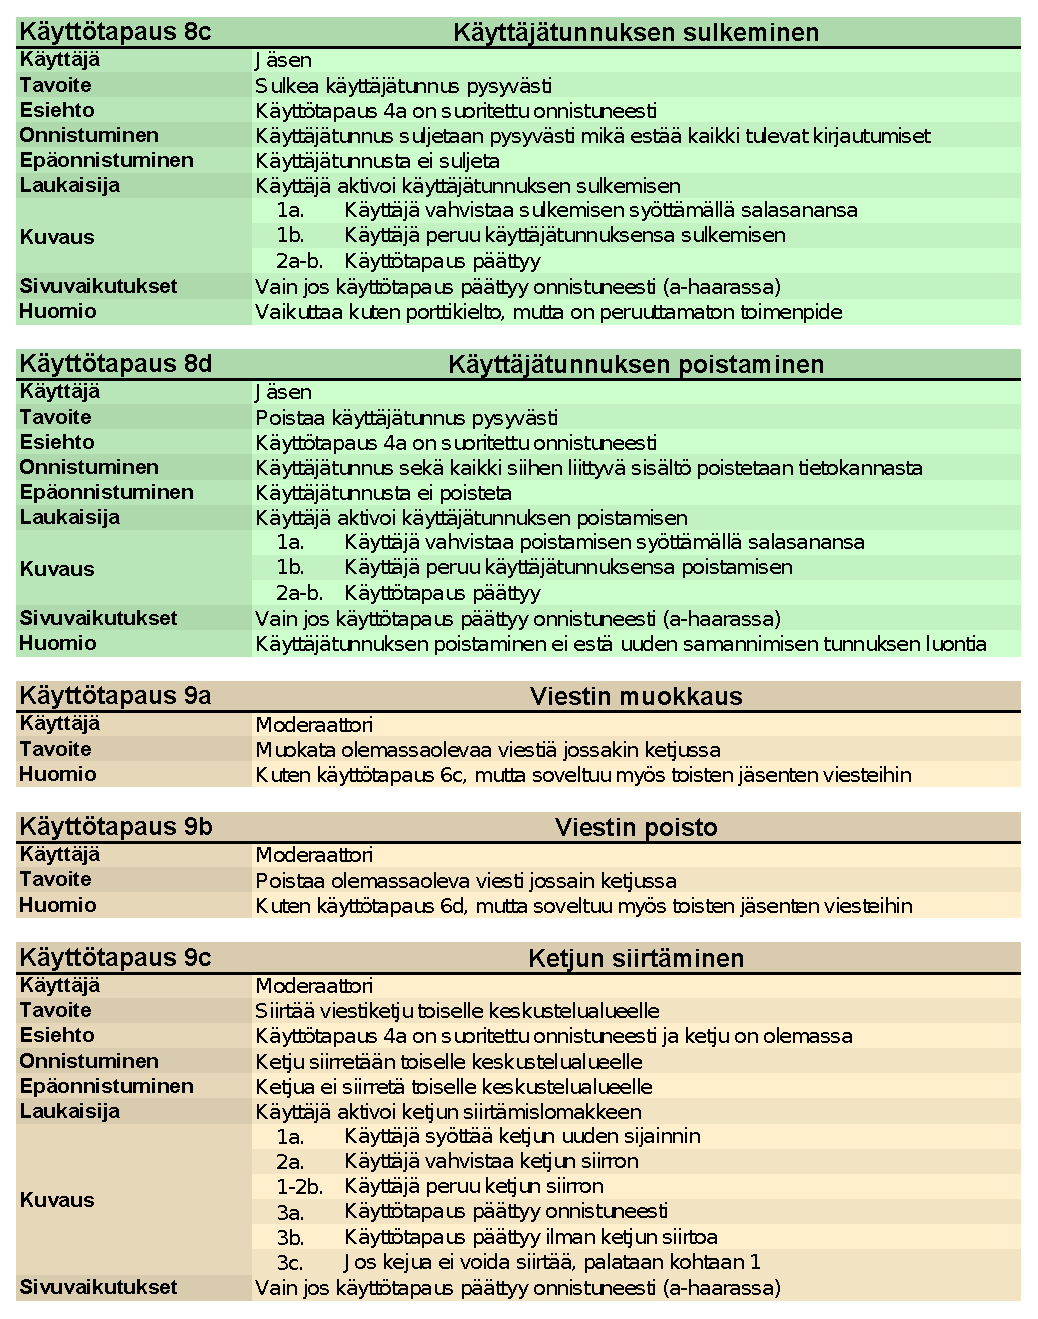
\includegraphics[trim = 21mm 0mm 0mm 25mm]{kayttotapausmalli-sivu-4.eps}\\
		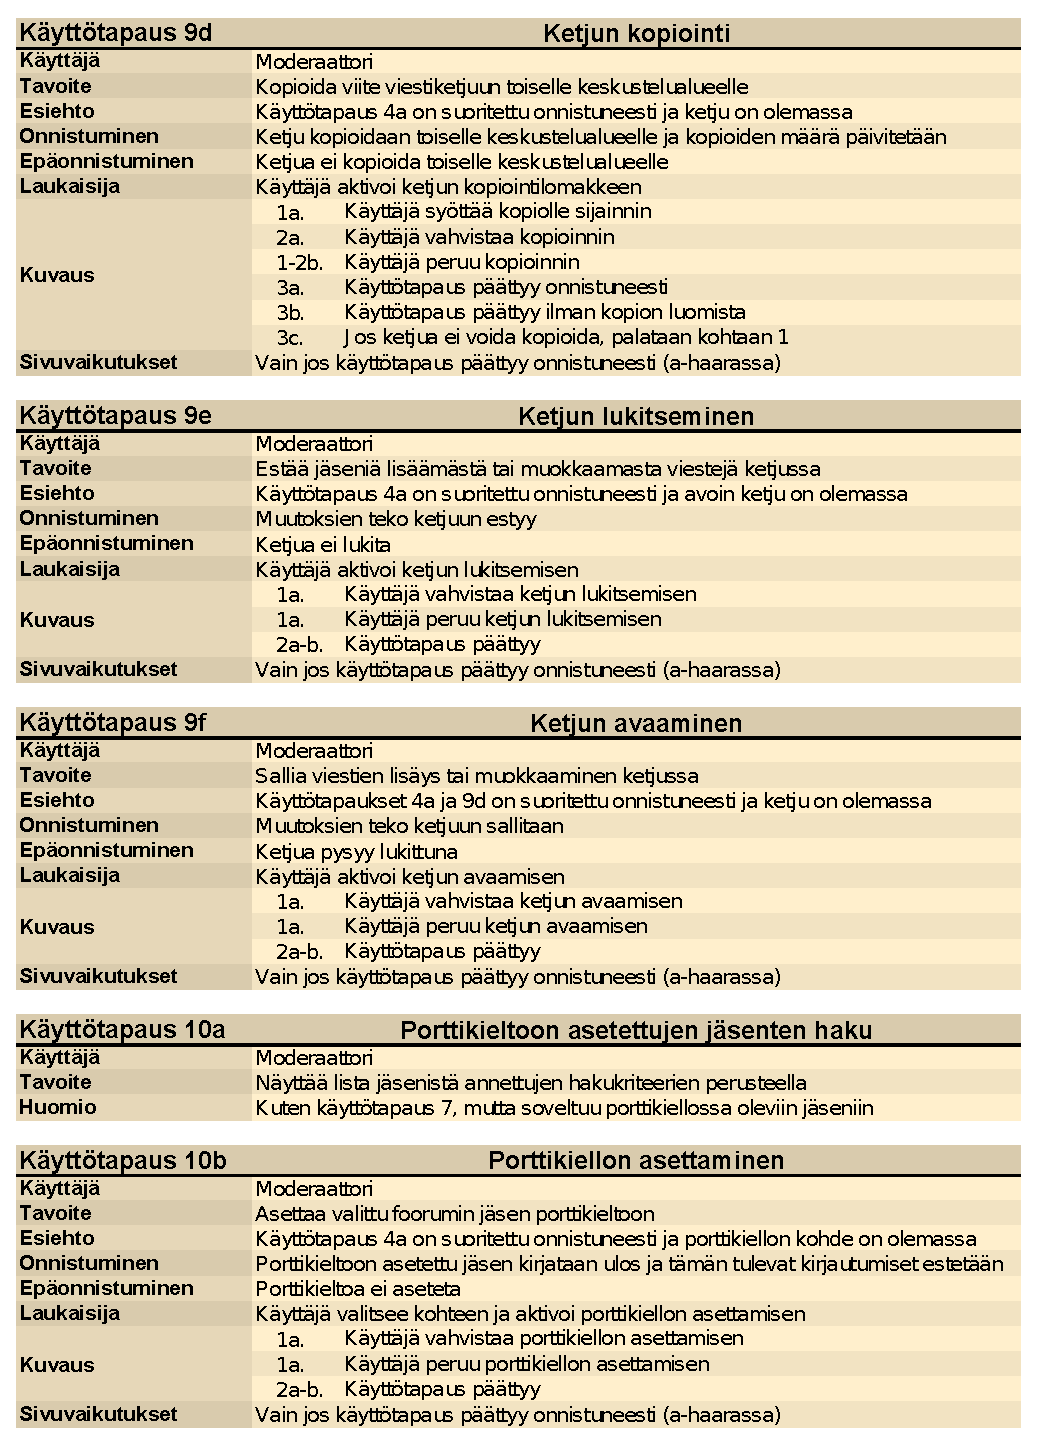
\includegraphics[trim = 21mm 0mm 0mm 25mm]{kayttotapausmalli-sivu-5.eps}\\
		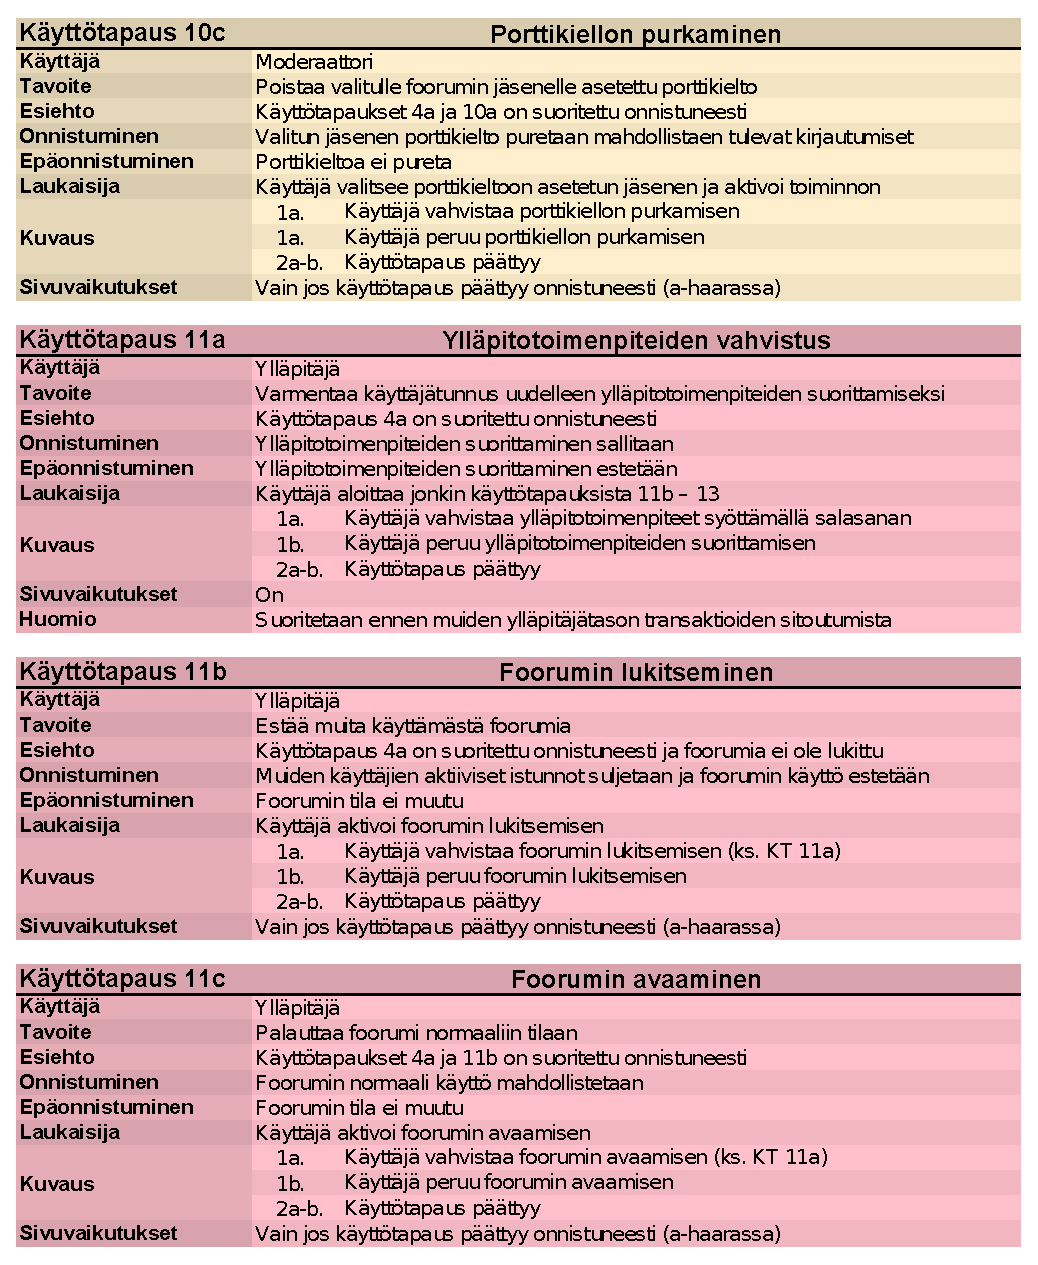
\includegraphics[trim = 21mm 0mm 0mm 25mm]{kayttotapausmalli-sivu-6.eps}\\
		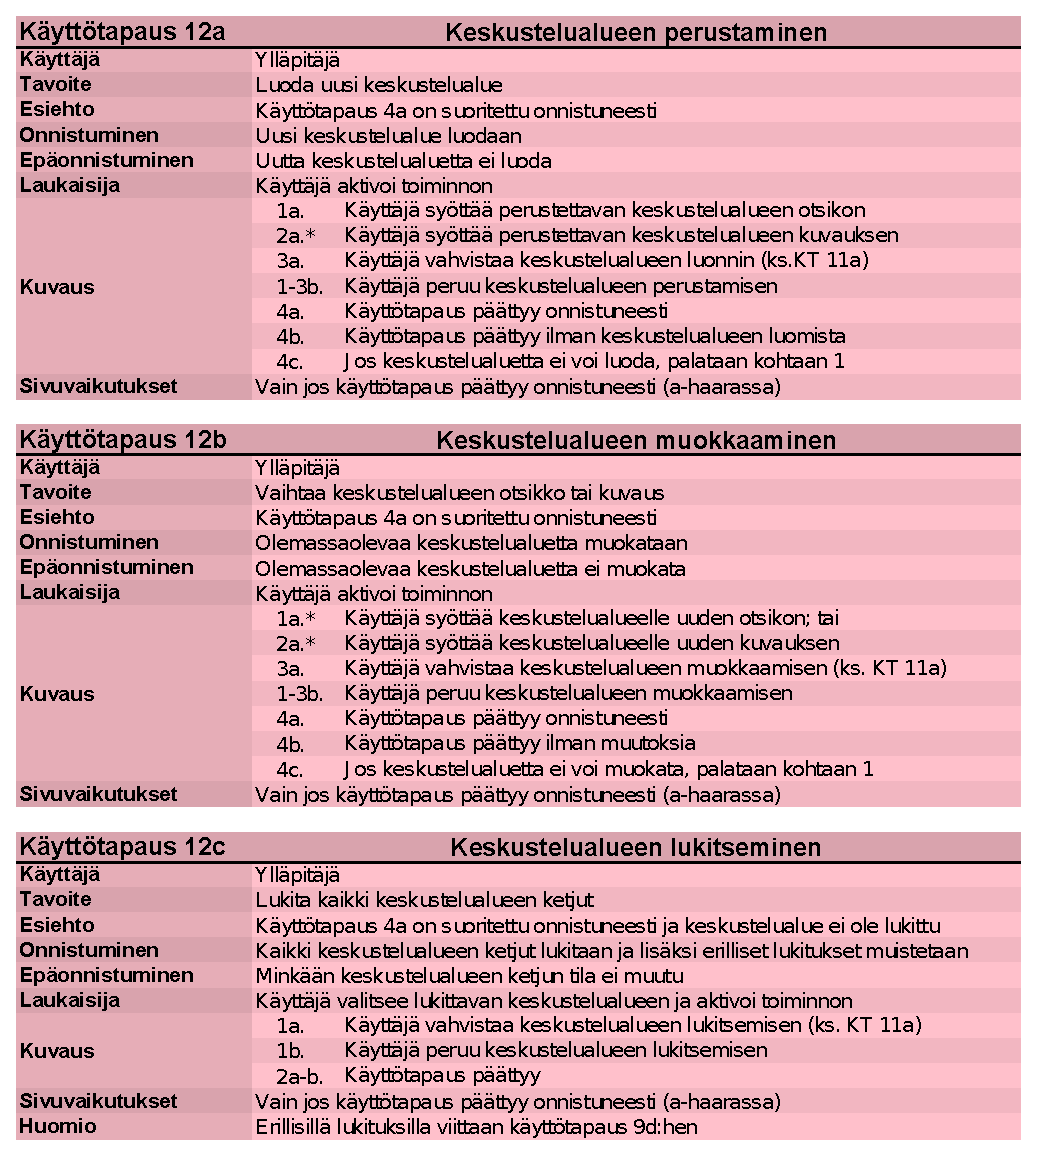
\includegraphics[trim = 21mm 0mm 0mm 25mm]{kayttotapausmalli-sivu-7.eps}\\
		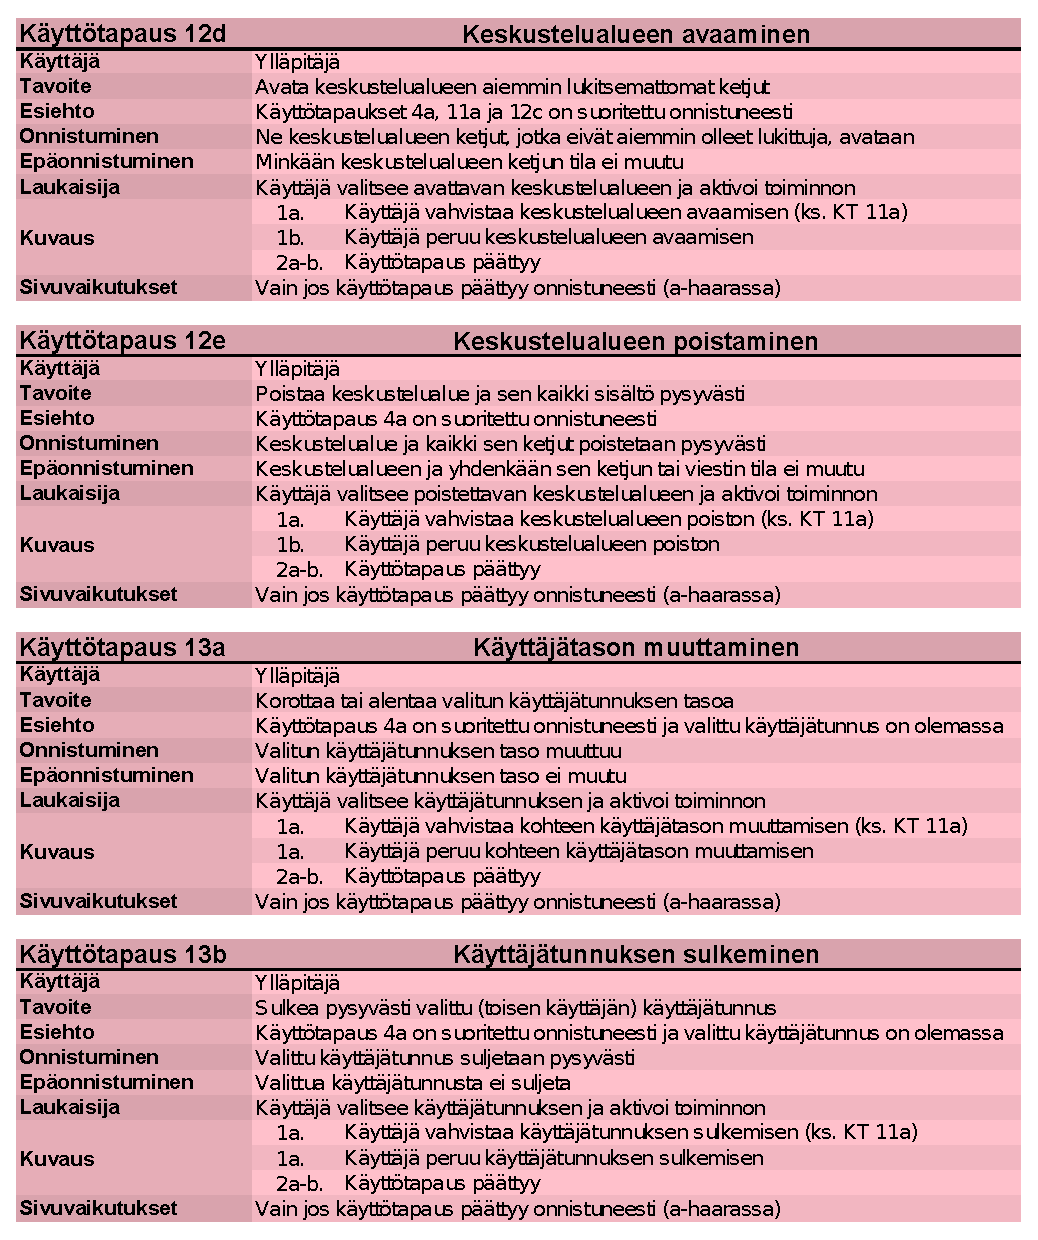
\includegraphics[trim = 21mm 0mm 0mm 25mm]{kayttotapausmalli-sivu-8.eps}\\
		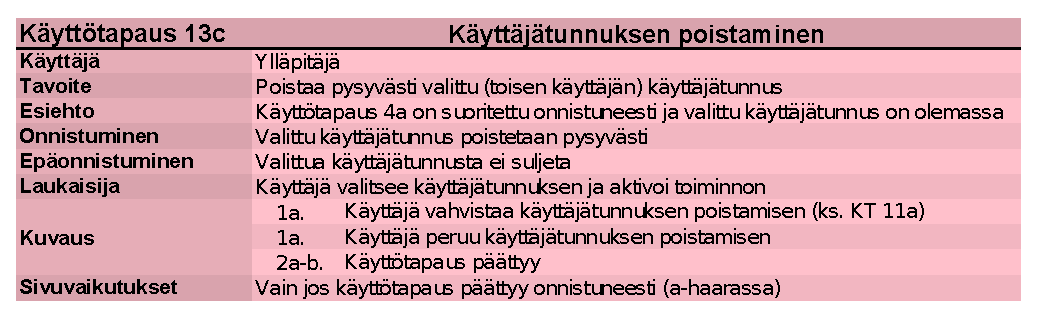
\includegraphics[trim = 21mm 0mm 0mm 25mm]{kayttotapausmalli-sivu-9.eps}\\
		
		% Ylläolevat lasken "yhdeksi" kuvaksi...
		\begin{figure}
			\caption{Käyttötapausmalli}
		\end{figure}

\newpage
\thispagestyle{plain}
\section{Tietosisältö}
	\subsection{Tietovaatimukset}
		Edellisessä kappaleessa esittämäni foorumin yleiskuvan perusteella olen päätynyt siihen tulokseen,
		että järjestelmässä on neljä varsinaista yksilötyyppiä. Yksilötyy-pit ovat \emph{jäsen, viesti, ketju}
		ja \emph{keskustelualue}. Vierailijoille ei tarvita mitään tauluja tietokannassa sillä nämä eivät
		voi tuottaa sisältöä foorumille (vaikka voivatkin esimerkiksi lukea viestitauluja).		
		
	\subsection{Käsitekaavio} Alla on käsitekaavio keskeisimmistä tietokohteista:
		\begin{figure}[H]		
			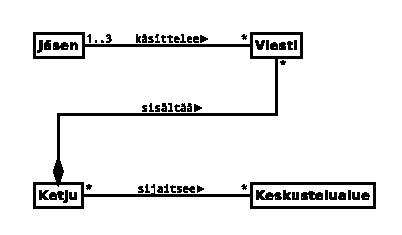
\includegraphics[trim = 0mm 0mm 0mm -3mm, scale = 2.0]{kasitekaavio.eps}
			\caption{Käsitekaavio}
		\end{figure}	
		
	\subsection{Tietokohteet} Seuraavalla sivulla olen listannut lyhyen taulukkomuotoisen kuvauksen edellä
		esi-tetyistä tietokohteista. Arvojoukolla merkkijono($n$) viittaan vaihtuvan mittaisiin korkeintaan
		$n$ merkkiä pitkiin merkkijonoihin.
	
		\newpage
		\thispagestyle{plain}
		
		\begin{figure}[H]
			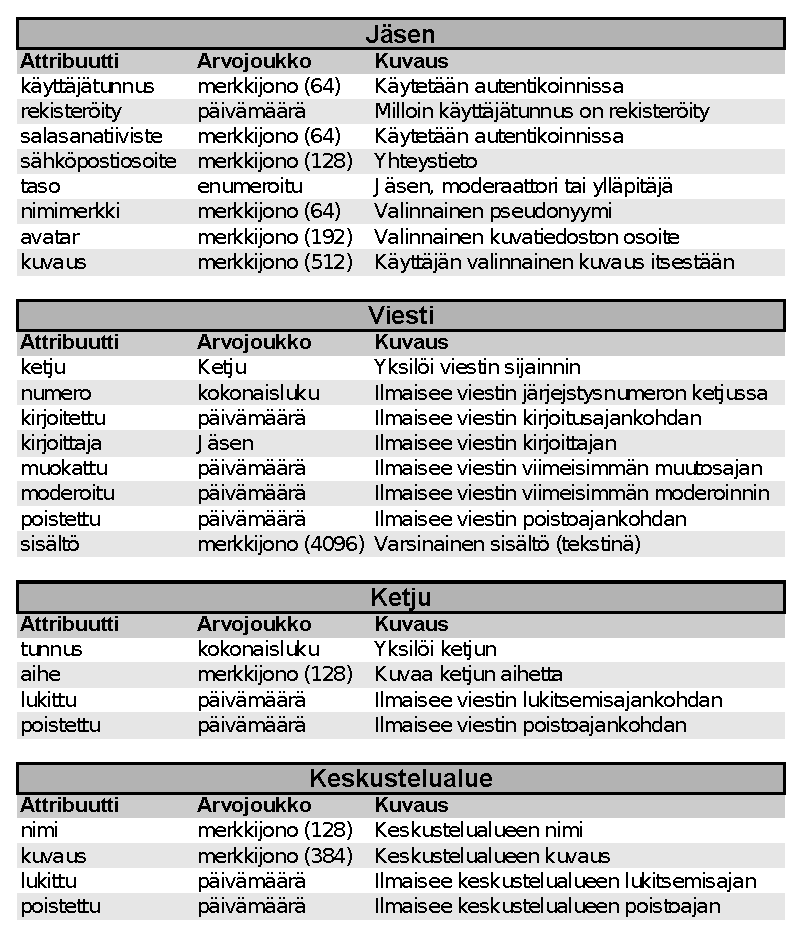
\includegraphics{tietokohteet.eps}
			\caption{Tietokohteet}
		\end{figure}
		
\newpage
\thispagestyle{plain}		
	\section{Relaatiotietokantakaaviot}
		\subsection{ER-kaavio} Seuraavalla sivulla on tietokannan riippuvuuksia korkealla tasolla kuvaava
		ER-kaavio. Olen esittänyt siinä kohteiden tyypit väreillä, mikä ilmenee kuvassa ole-vasta selityksestä.
		Lisäksi selvennettäköön, että olen tilan säästämiseksi esittänyt tietotyypin "Jäsen" valinnaiset
		attribuutit moniarvoisena attribuuttina "muut" se-kä viitannut porttikiellon asettamiseen potkimisena.
		
		\subsection{UML-kaavio} Olen myös laatinut tarkemman kaavion, josta ilmenee kaikki varsinaiseen
		tie-tokantaan luotavat taulut attribuutteineen ja avaimineen. UML-kaavio on sivulla 21. Olen merkinnyt
		ensisijaiset ja vierasavaimet stereotyypein $<<$PK$>>$ ja $<<$FK$>>$. Lisäksi olen värittänyt
		kaavioon varsinaisia yksilötyyppejä vastaavat taulut sinisellä, heikkoja yksilötyyppejä vastaavat
		taulut punaisella sekä muut taulut vihreällä taustavärillä.
		
		\newpage
		\thispagestyle{plain}
		\begin{figure}[H]		
			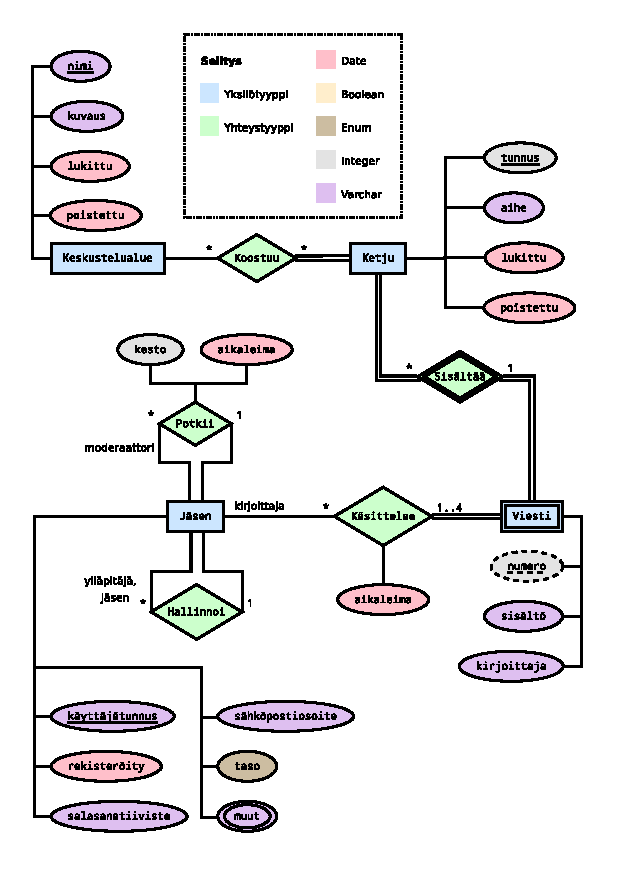
\includegraphics[trim = 6mm 0mm 0mm 20mm, scale = 1.5]{er-kaavio.eps}
			\caption{ER-kaavio}
		\end{figure}
		
		\newpage
		\thispagestyle{plain}
		\begin{figure}[H]		
			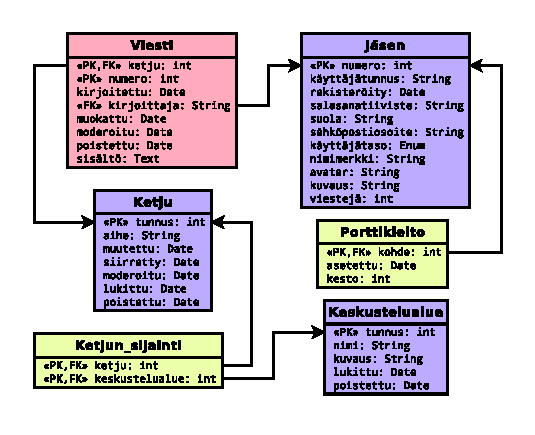
\includegraphics[trim = 0mm 0mm 0mm 20mm, scale = 1.5]{uml-tietokantakaavio.eps}
			\caption{Tietokantakaavio}
		\end{figure}
		
\newpage
\thispagestyle{plain}
	\section{Järjestelmän yleisrakenne}
	
\newpage
\thispagestyle{plain}
	\section{Käyttöliittymä}
		\subsection{Käyttöliittymäkaavio} Seuraavalla sivulla näkyvä kaavio antaa yleiskuvan käyttöliittymän
		komponenteista ja niiden välisistä suhteista. (Päivitän komponenttien lopulliset tiedostonimet näkyviin
		myöhemmin.) Esityksen selkeyttämiseksi olen värikoodannut komponentit niiden käyttöön tarvittavaa
		pienintä käyttäjätasoa vastaavalla väril-lä aiempaa käytäntöäni vastaavasti. (Toisin sanoen kaikkien
		käytettävissä olevat komponentit ovat sinisiä, jäsenten käytettävissä olevat vihreitä, moderaattoreiden
		keltaisia sekä ylläpitäjän punaisia.) Lisäksi on syytä huomata että joihinkin komponentteihin liittyy
		lisätoiminnallisuutta korkeammilla käyttäjätasoilla. Esi-merkiksi komponentti "Käyttäjätunnus" tarjoaa
		ylläpitäjälle palvelun, joka mahdollistaa kohteena olevan käyttäjätunnuksen käyttäjätason muuttamisen.
		
		\newpage
		\begin{figure}[H]		
			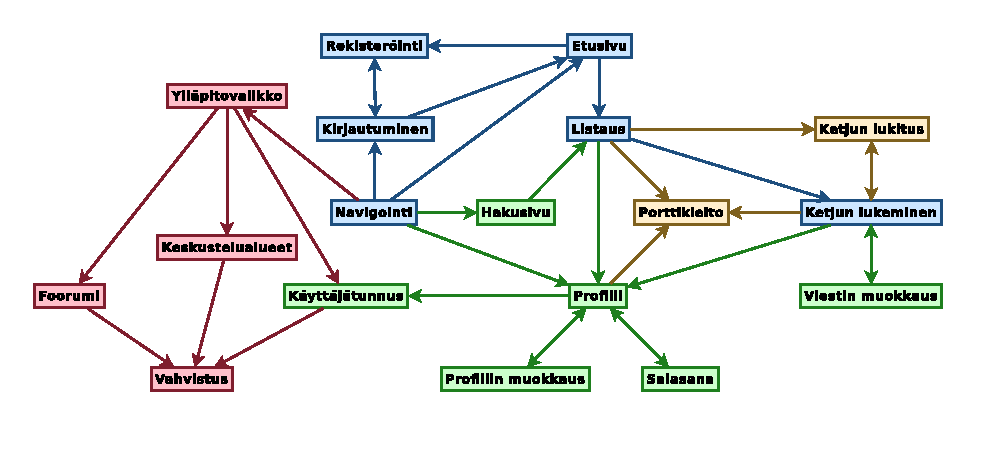
\includegraphics[trim = 0mm 0mm 23mm -7mm, scale = 1.5, angle = 90]{kayttoliittymakaavio.eps}
			\caption{Käyttöliittymäkaavio}
		\end{figure}

%\newpage
%\section{Relaatiotietokantakaavio}
	
\end{document}